\chapter{Architettura di Dropper}
\label{cap:architettura}

In questo capitolo si fa una descrizione dettagliata dei requisiti e
delle funzionalità presenti nell'architettura designata per lo
sviluppo di Dropper.

L'obiettivo di Dropper è quello di generare, analizzando un file
oggetto eseguibile, il payload corrispondente ad una catena di gadget
che se iniettato nello stack dell'immagine del processo associato a
quell'eseguibile, consente di prenderne il controllo, eseguendo un
comando arbitrario sulla macchina. Lo strumento applica tecniche note
per eludere misure di protezioni esistenti come la casualizzazione
degli indirizzi (\lstinline{ASRL}), stack e aree dati non eseguibili
(``W $\oplus$ X'') o la read-only relocation, automatizzando il più
possibile la scelta della strategia appropriata. 

Dropper analizza il binario utilizzando alcune delle funzionalità del
recente framework per l'analisi dei binari \lstinline{BARF}
\cite{Heitman-14}. Il linguaggio utilizzato per la scrittura di
Dropper è python e, nella sua prima versione, supporta le architetture
\lstinline{x86} e \lstinline{x86-64} su piattaforme GNU/Linux (il
formato degli eseguibili supportato è ELF). Tuttavia come tratteremo
meglio nel corso di questo capitolo, queste restrizioni possono essere
facilmente superate nelle future versioni grazie all'astrazione data
dall'utilizzo di un linguaggio intermedio per rappresentare le
istruzioni.

Una tipica sessione dell'utilizzo di Dropper può essere
grossolanamente divisa in quattro fasi:

\begin{enumerate}
\item Analisi del binario 
\item Estrapolazione e analisi dei gadget
\item Scelta della strategia da utilizzare
\item Creazione del payload
\end{enumerate}

Nella prima fase, quella in cui si analizzano le informazioni presenti
nel file oggetto eseguibile esaminato, vengono ricavate le
informazioni sulle misure di protezione attualmente in uso sul file
oggetto eseguibile, le funzioni utilizzate e le librerie dinamiche
importate. Queste informazioni verranno utilizzate specialmente nella
terza fase.

Dropper, nella seconda fase, ricerca all'interno del file binario i
gadget disponibili. I gadget trovati vengono tradotti, dal framework
BARF, in un linguaggio intermedio: REIL
\cite{dullien-09}. Effettuare le analisi su un linguaggio
intermedio anziché sulle istruzioni dell'architettura vera e propria
porta una serie di vantaggi:

\begin{itemize}
 \item le operazioni di analisi vengono astratte e rese
   indipendenti dalla specifica architettura. In questo modo è
   possibile aggiungere il supporto di altre architetture allo
   strumento in modo molto più semplice, operazione che si riduce a
   sviluppare un traduttore da questa architettura al linguaggio
   intermedio

 \item REIL ha un insieme di istruzioni molto ridotto (solo
   quattordici istruzioni), questo facilità notevolmente lo sviluppo
   di strumenti di analisi

  \item le istruzioni di REIL non presentano nessun effetto
  secondario implicito, come invece avviene per la maggior parte delle
  istruzioni delle architetture reali

\end{itemize}

Una volta trovati e tradotti in un linguaggio intermedio è necessario
estrapolare la semantica dei gadget. Questo permetterà nella fase
successiva l'assemblaggio di piccole catene che consentano di eseguire
operazioni particolari (come modificare il valore dello stack,
chiamare una funzione, settare un registro, scrivere in memoria,
operazioni aritmetiche, leggere dalla memoria, ecc). Dropper
utilizzerà nella fase di creazione del payload queste piccole catene
per assemblare catene via via più lunghe che eseguono operazioni più
complesse e articolate. L'architettura prevede che la generazione di
queste sequenze avvenga sia in maniera programmatica, in cui la
procedura per la sua costruzione è codificata in un algoritmo, sia in
maniera dichiarativa, ad esempio utilizzando linguaggi di planning
come \lstinline{PDDL}\cite{pddl-97}. Un analisi sui vantaggi e sui
problemi che si incontrano in una codifica del genere è riportata
nella sezione \ref{sec:pddl}.

Nella terza fase, per scegliere la tecnica di exploit appropriata,
Dropper si basa sia su alcune informazioni che fornisce l'utente in
merito all'errore che si sta sfruttando (ad esempio se può controllare
un file descriptor, se ci sono limiti nella dimensione del payload o
nei caratteri ammessi) sia su quelle ricavate dalla prima fase di
analisi dell'eseguibile. Dev'essere semplice estendere Dropper con
nuove strategie.

L'ultima fase si occupa di assemblare gli indirizzi dei gadget e
valori concreti per la generazione di un payload che, una volta
iniettato sullo stack, comporti l'esecuzione delle varie catene
assemblate nelle fasi precedenti.

%% Una volta codificato il
%% problema in questi termini si può chiedere ad un planner, come se
%% fosse una sorta di oracolo, in che sequenza collegare le varie azioni
%% (cioè le varie sequenze elementari di gadget) per ottenere quello
%% stato. La rappresentazione delle informazioni sulla semantica dei
%% gadget è espressa in questo modo in forma esplicita, e non più
%% codificata in un algoritmo.

\begin{figure}
\begin{center}
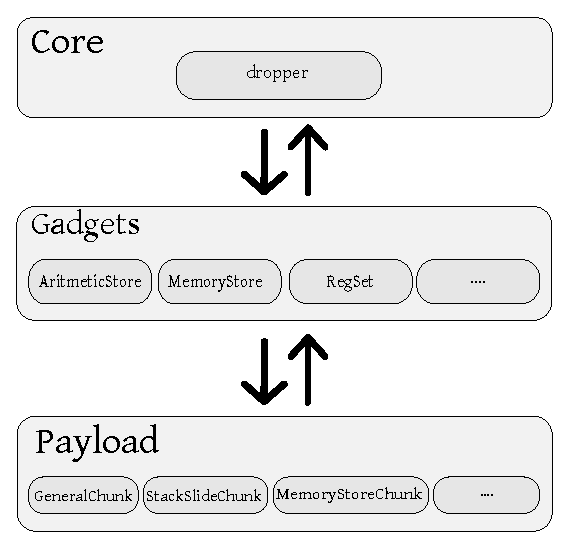
\includegraphics{img_architettura}
\caption{Architettura di Dropper}
\label{fig:arch}
\end{center}
\end{figure}

L'architettura di Dropper si compone di tre moduli logici,
rappresentati in figura \ref{fig:arch}:

\begin{itemize}

  \item Core: È il modulo che si occupa di 
    \begin{inparaenum}[a)] 
      \item leggere il binario,
      \item coordinare le operazioni dei restanti moduli,
      \item interagire con l'utente per ottenere informazioni
        aggiuntive sul binario e/o sullo scenario nel quale dev'essere
        prodotta la catena e 
      \item scegliere la strategia di exploit più appropriata
    \end{inparaenum}
  \item Gadgets: È il modulo che si occupa dell'estrapolazione,
    dell'analisi, della scelta e dell'assemblaggio dei gadget da utilizzare nella
    composizione della catena e dei vari sui frammenti

  \item Payload: È il modulo che si occupa di trasformare una
    sequenza ordinata di gadget in un payload vero e proprio da
    iniettare sullo stack, gestendo il posizionamento corretto degli
    indirizzi e dei valori utilizzati dai vari gadget

\end{itemize}

\section{Modulo Core}
\label{sec:arc:core}

È il modulo che si occupa di leggere il file binario, interagire con
l'utente, scegliere le varie strategie da adottare e di coordinare le
azioni degli altri moduli. 

Dropper parsa l'ELF e ricava la lista delle funzioni che il file
oggetto eseguibile utilizza, i relativi elementi nella \emph{Procedure
  Linkage Table} (vedi \ref{sec:plt}), le aree di memoria all'interno
dell'immagine del processo dove è possibile scrivere e da dove è
possibile leggere e le misure di protezione utilizzate dal file
binario. Per il parsing dell'ELF Dropper utilizza una libreria
apposita, pyelftools (\cite{pyelftools}).

L'utente poi, interagendo con il modulo, fornisce informazioni
aggiuntive necessarie alla generazione della catena e linee guida
sulla strategia da utilizzare. Tra le informazioni che può fornire
l'utente troviamo:

\begin{itemize}
  \item La possibilità da parte dell'utente di controllare un file
    descriptor
  \item I file oggetto condivisi utilizzati dall'eseguibile sulla
    macchina dove si intende far eseguire la catena. Questi file
    vengono analizzati al fine di ricavarne gli offset da utilizzare
    nelle tecniche di sovrascrizione della GOT (vedi
    sez. \ref{sec:expl})
  \item Eventuali caratteri che non possono comparire all'interno del
    payload
  \item Eventuali limiti sulla lunghezza del payload
  \item Il comando da eseguire
\end{itemize}

Con tutte queste informazioni il modulo può quindi procedere nello
stabilire quale strategia utilizzare e richiedere al modulo
Gadgets le sequenze di gadget necessarie. Lo schema principale
delle varie strategie, si può dividere in due fasi: 

\begin{inparaenum}[1)]
\item preparare e scrivere in memoria gli argomenti per eseguire una
  chiamata ad una funzione di libreria che ci consenta di eseguire un
  comando arbitrario (\lstinline{execve} o \lstinline{system}) e
\item eseguire quella
funzione.
\end{inparaenum}

Per scrivere in memoria è possibile utilizzare diverse strategie,
Dropper deve scegliere la più adatta o quella specificata
dall'utente. Il modulo deve essere facilmente estendibile per
aggiungere nuove strategie. Alcune delle strategie più efficienti per
scrivere in memoria sono:

\begin{itemize}

\item Nel caso sia possibile inserire arbitrariamente dei valori in un
  file descriptor (ad esempio se l'utente può inserire uno stream di
  dati nell'input del programma) allora è comodo utilizzare la
  funzione \lstinline{read} della \lstinline{libc} per copiare questi
  dati nell'area di memoria di destinazione. Dropper fornisce i valori
  da ``inserire'' nello stream dati del file descriptor. L'attaccante
  deve fare in modo che quando la funzione \lstinline{read} venga
  richiamata siano letti dal file descriptor proprio quei dati

\item Utilizzo di catene di gadget che consentano di scrivere valori
  costanti in memoria. Per poter utilizzare questa tecnica devono
  essere disponibili i gadget delle categorie necessarie, in più i
  valori da caricare in memoria non devono presentare caratteri che
  non possono essere presenti nel payload. In questa tecnica i dati
  non vengono scritti tutti in insieme ma a chunk di alcuni bytes per
  volta (a seconda dell'architettura o del tipo di gadget). A seconda
  del tipo di gadget per ognuna di queste iterazioni è necessario
  inserire nel payload un certo numero di bytes di ``padding''. Per
  questi motivi l'utilizzo di questa tecnica tende a generare payload
  piuttosto lunghi

\item Utilizzo delle funzioni \lstinline{strcpy} o \lstinline{memcpy}
  per copiare byte presenti in posizioni note all'interno
  dell'eseguibile nella posizione desiderata \cite{longld:2010}.
  Questa tecnica, copiando verosimilmente solo un byte per volta tende
  anch'essa a generare payload abbastanza lunghi ma ha il grande
  vantaggio di poter copiare anche valori che non possono essere
  presenti nel payload. È necessario che i valori dei byte che voglio
  copiare siano già presenti nell'eseguibile, condizione che, a meno
  di file oggetto eseguibili molto piccoli, risulta abbastanza comune

\item Nel caso si riesca ad ottenere in qualche modo (ad esempio
  attraverso una seconda vulnerabilità) la conoscenza dell'indirizzo
  dello stack i valori possono essere inseriti direttamente insieme al
  payload

\end{itemize}

Una volta scritti gli argomenti per la funzione da richiamare in
memoria è necessario chiamare la funzione stessa. La funzione deve
permetterci di eseguire un comando arbitrario. All'interno della
\lstinline{libc} sono presenti due funzioni con queste
caratteristiche: \lstinline{execve} e \lstinline{system}. Un ritorno
diretto alla funzione solitamente non può avvenire, in quanto il
valore del suo indirizzo in memoria è casualizzato. Tuttavia, se una
di queste due funzioni è utilizzata all'interno del programma, basterà
ritornare al suo elemento nella Program Linkage Table, che ha una
posizione nota e fissa all'interno della memoria dell'immagine del
processo. Se così non fosse un'alternativa è quella di adoperare
tecniche per ricavare l'indirizzo della funzione partendo
dall'indirizzo di un'altra funzione della stessa libreria che invece
viene utilizzata dal programma. Alcune considerazioni su queste
tecniche, descritte nella sezione \ref{sec:expl}, che riguardano
l'architettura di Dropper sono:

\begin{itemize}
  \item Devono essere noti gli offset tra le funzioni all'interno del
    file oggetto condiviso della libreria utilizzato sulla macchina
    bersaglio. L'utente può fornire a Dropper un file di questo tipo
    dal quale verranno ricavati i relativi offset. È da notare che,
    variando in un range relativamente piccolo, non dovrebbe essere
    impossibile, se le condizioni lo consentono, montare un attacco di
    tipo forza bruta per ricavare questi offset

  \item Come visto in \ref{sec:expl} per poter utilizzare la tecnica
    di GOT patching il binario deve presentare una sequenza di gadget
    che ci consenta di eseguire un'operazione di somma (o
    un'operazione che ci consenta di simulare una somma, come una
    sottrazione) tra un offset di tre/quattro byte e un'area di
    memoria arbitraria (l'area dove è memorizzato l'indirizzo della
    funzione usata come riferimento, solitamente nella GOT). Molto
    spesso però abbiamo gadget che ci consentono di addizionare solo
    un byte per volta. Questo è un problema perché in un'operazione di
    somma byte per byte dev'essere considerato un eventuale valore di
    riporto tra un byte e il successivo. Un modo per risolvere questo
    problema è utilizzare gadget che utilizzino un'istruzione di tipo
    \lstinline{adc} (add with carry), facendo attenzione che gli
    effetti secondari degli altri gadget coinvolti nella catena non
    vadano a modificare il carry flag. Quest'istruzione viene
    utilizzata proprio per le addizioni multi-byte e aggiunge anche il
    valore del carry flag quando esegue l'operazione di somma. In
    realtà anche non avendo a disposizione questo tipo di gadget, per
    via dell'allineamento in memoria, gli ultimi bit dell'indirizzo di
    una funzione non variano tra un'esecuzione e la successiva. Con
    questa parziale conoscenza del valore iniziale si può comunque
    creare una catena con un alta percentuale di successo come
    descritto nella sezione \ref{sec:arithmeticstore}
\end{itemize}

È interessante notare come, anche se vi è una guida nelle operazioni
da seguire basata sulla strategia scelta, la sequenza di operazioni
che conducono allo stato del sistema desiderato sono molteplici. Ad
esempio l'operazione aritmetica per il calcolo dell'indirizzo della
funzione bersaglio potrebbe avvenire in memoria, oppure tra due
registri e poi salvata in memoria. Qui si notano i vantaggi che
potrebbe avere un approccio che modelli la situazione in un problema
di planning rispetto ad un approccio di tipo programmatico. Infatti,
con un approccio programmatico, tutte le combinazioni vanno codificate
nell'algoritmo, una procedura la cui completezza è più difficile da
dimostrare e che è molto più soggetta ad errori.

\subsection{Utilizzo di pianificatori}
\label{sec:pddl}

Il problema di generare una catena (quindi una sequenza) di gadget
(che possono essere visti come azioni) per arrivare ad uno stato del
sistema desiderato si traduce naturalmente in un problema di
planning. Una volta tradotto si può utilizzare un planner per ottenere
una soluzione valida e/o (dipende dal planner che si utilizza)
ottima.

Nel 1998 Drew McDermott rilascia il Planning Domain Description
Language (PDDL) \cite{pddl-97,fox-03}, un linguaggio che ha come
obiettivo quello di fornire uno strumento universale per codificare
problemi di planning. In questa sezione esamineremo un primo approccio
che può essere utilizzato per tradurre alcuni dei problemi affrontati
da Dropper nel linguaggio PDDL, analizzandone le principali
problematiche. Il linguaggio PDDL è fatto in modo da separare la
descrizione del dominio del problema da quella della singola istanza.

Gli elementi che possono essere descritti all'interno della codifica
del dominio del problema rilevanti al fine della nostra discussione sono:
\begin{itemize}
\item I diversi tipi di oggetto presenti nel nostro dominio
\item \emph{Costant}, cioè oggetti che sono presenti in tutte le istanze del problema
\item \emph{Fluent}, mapping tra una tupla di oggetti e un valore
  numerico che può cambiare durante un piano. La loro sintassi e
  semantica è stata stabilizzata nel linguaggio in \cite{fox-03}
\item \emph{azioni}. Ogni azione può avere dei parametri e definisce
  l'insieme delle possibili modifiche che possono essere effettuate
  nel dominio modellato. Per ogni azione si indicano le precondition
  (ovver condizioni necessarie per effettuare un'azione) e gli effetti
  che le azioni hanno sugli oggetti del dominio o su i fluent
\end{itemize}

Una singola istanza del problema invece definisce gli oggetti che le
azioni possono manipolare, lo stato iniziale nel quale si trova il
sistema, lo stato che vogliamo raggiungere (il nostro ``goal'') e
la metrica con la quale valutare la bontà di un piano.  Come
evidenziato in \cite{fox-03} i fluent non possono essere utilizzati
come parametri di azioni perché queste agiscono su oggetti ``fisici''
e quindi i parametri devono appartenere ad insiemi finiti (e non ad
insiemi infiniti come i numeri). 

Per ovviare a questa limitazione nella nostra modellazione
utilizzeremo come stratagemma quello di creare degli oggetti di tipo
\lstinline{imm} e di associargli un valore tramite il fluent
\lstinline{val (?x - imm)}. Questo fa si che le azioni possono
utilizzare parametri di tipo \lstinline{imm} e che negli effetti
possiamo ricavare il valore che l'oggetto di tipo \lstinline{imm}
rappresenta. Questo ci obbliga, nell'istanza del problema, a definire
tutti i valori numerici che saranno presenti nel piano come oggetti di
tipo \lstinline{imm} e ad associare per ognuno di essi il relativo
fluent.

I tipi di dato utilizzati nella modellazione sono \lstinline{imm}, con
il significato appena spiegato, e \lstinline{register} che rappresenta
per l'appunto un registro. I fluent utilizzati invece sono:

\begin{itemize}
\item \lstinline{(val ?x - imm)} come appena definito
\item \lstinline{(reg ?r - register)} che rappresenta il valore attuale del
  registro ?r
\item \lstinline{(mem ?a - imm)} che rappresenta il valore attuale
  della locazione di memoria \lstinline{?a}
\end{itemize}

Vengono create tante costanti quante i registri.  Ogni azione invece
corrisponde ad un gadget e le azioni riflettono gli effetti che il
gadget ha su i registri e sulla memoria.  Attualmente si è proceduto a
modellare solo gadget per l'impostazione di registri o la scrittura di
memoria. È da notare che per lo stratagemma usato tutti i valori
(indirizzi e valori concreti) che le nostre azioni vanno ad utilizzare
devono essere esplicitati. Un gadget per l'impostazione di un registro
viene tradotto in questo modo (a meno dei puntini utilizzati per
generalizzare la lista dei registri):

\begin{lstlisting}
  (:action regset_gadget
	 :parameters (?vreg0 ?vreg1 ... ?vregn - imm)
	 :precondition (and)
	 :effect (and
	 	 (assign (reg reg0) (val ?vreg0))
	 	 (assign (reg reg1) (val ?vreg1))
                 ...
	 	 (assign (reg regn) (val ?vregn))
		 (increase (stack-length) g.stack_offset)))
\end{lstlisting}

Come si può notare la traduzione avviene ad un livello d'astrazione
più alto delle singole istruzioni del gadget, dettagli come la
posizione dei valori da impostare nello stack, gli effetti secondari,
vengono gestiti sempre da Dropper. La traduzione invece di un gadget
per la scrittura in memoria è leggermente più complicata:

\begin{lstlisting}
(:action memstr_gadget
  :parameters ()
  :precondition (and)
  :effect (and 
           (forall (?a -imm) 
             (when (= (val ?a) (reg rdi))
              (assign (mem ?a) (reg rsi))))
          (increase (stack-length) 0)))
\end{lstlisting}

Questa modellazione poco elegante è dovuta al non poter utilizzare i
fluent come argomenti per altri fluent.

Una volta tradotto il dominio, si deve anche tradurre un'istanza del
problema. Si specificano gli oggetti che faranno parte dell'istanza
del problema, cioè i valori che andremo ad utilizzare. Come stato
iniziale si impostano i fluent dei registri a zero, si assegnano i
rispettivi valori ai fluent di tipo \lstinline{(val ?v - imm)} e si
imposta anche il fluent \lstinline{stack-length} a zero, quest'ultimo
viene utilizzato come metrica per valutare la bontà del piano
trovato. Come stato desiderato si imposta o, nel caso si voglia
trovare un piano per impostare un insieme di registri, che i fluent
rilevanti di tipo \lstinline{(reg ?r)} abbiano i valori desiderati o,
nel caso invece si voglia trovare un piano per impostare alcune
specifiche locazioni di memoria, che i fluent del tipo \lstinline{(mem  ?a)}
 abbiano il valore corrispondente.

Un esempio, con solo un piccolo sottoinsieme dei gadge trovati
nell'eseguibile ls è riportato nelle figure \ref{pddl:domain} e
\ref{pddl:facts}. L'esempio è generato tramite la classe
\lstinline{planner}.

La codifica appena presentata è molto banale e presenta alcuni
problemi. Prima di tutto non considera i valori della memoria e dei
registri come vettori di bit. Una soluzione potrebbe essere quella di
modellare la granularità delle azioni (e dei fluent) al singolo
byte. Anche se questo non consentirebbe di modellare azioni che
effettuino operazioni di tipo bit a bit aumenterebbe di molto
l'espressività della modellazione proposta. 

Il secondo problema è che una quantità di azioni grande quanto il
numero di gadget presente nell'eseguibile rende l'utilizzo di planner
general-purpose inefficiente. Nei primi test effettuati la maggior
parte dei planner non riesce neanche a iniziare la fase di ricerca del
piano. Una soluzione potrebbe essere quella di filtrare i gadget in
una prima fase, in modo da fornire una quantità più limitata di azioni
nella descrizione del problema.


\begin{lstlisting}[caption=Descrizione del dominio relativo ad un 
    piccolo sottoinsieme dei gadget presenti in ls,label=pddl:domain]
;gadget: 
;0x412050 : pop rsi; pop r15; ret
;0x412052 : pop rdi; ret
;0x40ea2c : mov dword ptr [rdi], esi; ret

(define (domain dropper )
(:requirements :typing :fluents :conditional-effects)
(:types imm register)
(:constants rax rbx rcx rdx rdi rsi rbp rsp rip r8 r9 r10 r11 r12 r13 r14 r15 - register)

(:functions 
  (val ?x -imm)
  (reg ?r - register)
  (stack-length)
  (mem ?addres - imm))

(:action regset_412052
   :parameters (?vrdi - imm)
   :precondition (and)
   :effect (and         (assign (reg rdi) (val ?vrdi))
     (increase (stack-length) 8)))

(:action regset_412050
   :parameters (?vr15 ?vrsi - imm)
   :precondition (and)
   :effect (and         (assign (reg r15) (val ?vr15))
         (assign (reg rsi) (val ?vrsi))
     (increase (stack-length) 16)))

(:action memstr_40ea2c
  :parameters ()
  :precondition (and)
  :effect (and (forall (?a ?v -imm) 
      (when (and (= (val ?a) (reg rdi))
      (= (val ?v) (reg rsi))) (assign (mem ?a) (val ?v))))
     (increase (stack-length) 0)))
)
\end{lstlisting}



\begin{lstlisting}[caption=Descrizione del dominio relativo ad
    un'istanza del problema,label=pddl:facts]
(define (problem memset)
(:domain dropper)
(:objects v_32896 v_2 v_33153 v_3 - imm)
(:init
(= (val v_32896) 32896)
(= (val v_33153) 33153)
(= (val v_2) 2)
(= (val v_3) 3)
(= (reg rax) 0)(= (reg rbx) 0)(= (reg rcx) 0)(= (reg rdx) 0)(= (reg rdi) 0)
(= (reg rsi) 0)(= (reg rbp) 0)(= (reg rsp) 0)(= (reg rip) 0)(= (reg r8) 0)
(= (reg r9) 0)(= (reg r10) 0)(= (reg r11) 0)(= (reg r12) 0)(= (reg r13) 0)
(= (reg r14) 0)(= (reg r15) 0)
(= (mem v_32896) 0)
(= (mem v_33153) 0)
(= (stack-length) 0))
(:goal 
(and (= (mem v_32896) 2)
  (= (mem v_33153) 3)))
(:metric minimize (stack-length))
)
\end{lstlisting}


\section{Modulo Gadgets}

Il modulo Gadgets si occupa di ricavare i gadget presenti nel file
oggetto eseguibile, di estrapolarne la semantica e della creazione di
sequenze di gadget che se eseguite assolvono funzioni particolari
(come scrivere in memoria, settare un registro, ecc.). Questo modulo
interagisce con il modulo Payload per trasformare sequenze ordinate di
gadget in un payload vero e proprio da poter iniettare sullo stack ed
espone i metodi per la creazione delle catene che vengono usati dal
modulo Core.

Per la ricerca dei gadget all'interno del file oggetto eseguibile
viene utilizzata la classe \lstinline{GadgetFinder} del framework
BARF, che implementa al suo interno l'algoritmo
galileo\cite{Shacham-2007}.

%TODO descrivere galileo ?
%TODO utilizzare il nostro ?

Una volta disponibile l'insieme dei gadget presenti nel file oggetto
eseguibile bisogna, per ognuno di essi, estrapolarne la semantica. Per
estrapolarne la semantica si intende estrapolare in maniera automatica
gli effetti che una serie di istruzioni hanno sul contesto il quale,
semplificando, è rappresentato dalla memoria e dai registri della
macchina sulla quale saranno eseguite le istruzioni. Per questo tipo
di analisi si utilizzano due strumenti principali: la simulazione e la
traduzione delle istruzioni in un istanza di un problema SMT. 

\subsection{Traduzione di un gadget in formule logiche}

Un'istanza di un problema SMT può essere considerata come una formula
logica del primo ordine dove ad alcune funzioni e ad alcuni predicati
vengono assegnati significati e interpretazioni particolari
esplicitati in teorie aggiuntive \cite{Barrett-14}. Questo fa si che
possano essere sviluppati metodi decisionali costruiti su misura per
teorie specifiche, rendendo efficiente e possibile la codifica di
problemi di alcuni domini particolari. Ad esempio, considerando una
formula del tipo:

$$ x < y ∧ ¬(x < y + 0)$$

spesso ci interessa conoscere se la formula sia soddisfacibile solo
sotto i comuni significati delle funzione $+$, dei predicato $<$ e
della costante $0$, ovvero ci interessa conoscere la soddisfacibilità
della formula rispetto alla teoria aritmetica degli interi. Anche se è
possibile in ogni caso incorporare una serie di formule insieme a
quelle che descrivono un problmea in modo da forzare un risolutore
generale a considerare solo le interpretazioni compatibili con una
data teoria, le prestazioni computazionali ottenute in questo modo non
risultano spesso accettabili. Sono state sviluppate diverse procedure
su misura per molte teorie tra cui quella degli array e dei bitvector,
particolarmente rilevanti ai fini del nostro lavoro. Una volta che
sono a disposizione queste teorie risulta naturale modellare registri
e memoria rispettivamente attraverso Bitvector e Array di Bitvector.

Questi sono le motivazioni principali della scelta di una modellazione
che producesse un'istanza di un problema di SMT rispetto ad altri
metodi di modellazione logici come \emph{Answer Set Programming}.

Nelle figure \ref{cod:asm}, \ref{cod:reil} e \ref{cod:smt} sono
mostrate rispettivamente le istruzioni di un gadget per la scrittura
in memoria e le relative traduzioni in istruzioni REIL e in formule
SMT.

\begin{lstlisting}[caption=gadget per la scrittura in memoria, label=cod:asm]
mov dword ptr [rdi], esi
ret
\end{lstlisting}


\begin{lstlisting}[caption=traduzione del gadget in fig. \ref{cod:asm}
    nel linguaggio intermedio REIL, label=cod:reil]
str   [DWORD esi, EMPTY, DWORD t3]
stm   [DWORD t3, EMPTY, QWORD rdi]

add   [QWORD rsp, QWORD 0x8, QWORD t2]
str   [QWORD t2, EMPTY, QWORD rsp]
ret   [EMPTY, EMPTY, EMPTY]
\end{lstlisting}

\begin{lstlisting}[caption=traduzione del gadget in fig. \ref{cod:asm}
    in formule SMT, label=cod:smt]

(= ((_ extract 31 0) rsi_0) t3_1)
(= MEM_1 
  (store 
  (store 
  (store 
  (store MEM_0 (bvadd rdi_0 #x0000000000000000) ((_ extract 7 0) t3_1)) 
  (bvadd rdi_0 #x0000000000000001) ((_ extract 15 8) t3_1))
  (bvadd rdi_0 #x0000000000000002) ((_ extract 23 16) t3_1))
  (bvadd rdi_0 #x0000000000000003) ((_ extract 31 24) t3_1)))
(= t2_1 (bvadd rsp_0 #x0000000000000008))
(= t2_1 rsp_1)
\end{lstlisting}

Un'analisi completa della semantica presenta alcuni limiti dovuti alla
difficoltà di una modellazione completa del sistema nonché alla
conoscenza parziale del contesto (memoria e registri) reale in cui si
troveranno ad essere eseguite le istruzioni. Ad esempio utilizzando
l'attuale traduzione delle istruzioni in formule SMT, è difficile
porre al risolutore domande che riguardino il numero di letture
effettuate, o domandare se un'area di memoria viene mai letta. Per
quanto detto l'estrapolazione della semantica di un gadget avviene in
tre fasi descritte nelle prossime sezioni:
\begin{inparaenum}[a)]
\item emulazione e catalogazione, 
\item verifica e validazione e 
\item verifica degli effetti secondari.
\end{inparaenum}



\subsection{Emulazione e catalogazione}
La classe \lstinline{GadgetClassifier} del framework BARF emula il
gadget tenendo traccia delle operazioni sui registri e sulla
memoria. Con questi dati si verifica se il gadget appartiene ad una o
più categorie indicate in \cite{schwartz-2011}.
%TODO vanno elencate le categorie?  
Inoltre vengono identificati quali registri vengono utilizzati come
``operandi'' della funzione alla quale il gadget viene
associato. Basandosi su una simulazione, e quindi sull'analisi degli
effetti di solo un sottoinsieme dei possibili valori in ingresso,
questa catalogazione deve essere poi verificata con un'analisi
semantica vera e propria.

Le simulazioni vengono effettuate utilizzando dati concreti ma
un'esecuzione simbolica, funzionalità ancora non disponibile
all'interno del framework BARF, consentirebbe una catalogazione più
accurata esplicitando le relazioni tra i valori che i registri hanno
all'inizio e alla fine della simulazione o tra i valori iniziali dei
registri e gli accessi alla memoria.

\subsection{Verifica e validazione}
\label{sec:verifica_validazione}

Si deve poi verificare che, anche se il gadget esegua la funzione
della categoria alla quale viene assegnato, possa essere utilizzato
per i valori di tutto il ``dominio'' di questa funzione, cioè che non
ci siano restrizioni sugli operandi del gadget. Per esempio, un gadget
catalogato come \lstinline{MemoryStore} ma che utilizzi lo stesso
registro come operando di destinazione e operando sorgente non può
essere utilizzato per scrivere in una locazione arbitraria di memoria
un valore arbitrario in quanto il valore da scrivere e l'indirizzo di
memoria sono dipendenti tra di loro. In questa sezione ci riferiamo a
questa proprietà come alla ``generalità'' del gadget.

Bisogna verificare altresì che l'assegnamento dei valori appropriati
ai registri ``operandi'' sia condizione sufficiente perché il gadget
si comporti aderendo alla semantica della categoria in cui è stato
catalogato. Sempre continuando con l'esempio della scrittura in
memoria, questo vuol dire essere sicuri che, se i registri utilizzati
come operandi sono impostati con i valori appropriati, la scrittura in
memoria del valore voluto sia garantita per qualsiasi altra
combinazione iniziale dei restanti registri.

Queste due proprietà vengono verificate sia attraverso delle
simulazioni delle istruzioni nel linguaggio intermedio e sia
attraverso la sottomissione di istanze SMT ad un risolutore. Vengono
codificate per questi scopi due tipi di istanza SMT: una la quale
soddisfacibilità ci garantisce che un dato effetto può essere
realizzato (e viene anche fornito una configurazione del contesto che
porta a quell'effetto), e un'altra la quale non soddisfacibilità ci
garantisce che l'effetto del gadget aderisca alla semantica di
catalogazione per qualsiasi contesto iniziale. Istanze del primo tipo
possono essere utilizzate sia per ottenere la configurazione iniziale
con la quale ottenere un particolare effetto sul contesto, sia per una
verifica ``ottimista'' della generalità di un gadget (in questo caso
si utilizzano dei valori casuali e si assume che, se l'istanza è
soddisfacibile per alcuni valori casuali allora il gadget è generico).

Le istanze del primo tipo vengono create imponendo al modello che il
contesto finale rifletti l'effetto desiderato, quelle del secondo tipo
invece imponendo il complementare della condizione che rappresenta la
semantica che si sta cercando di verificare. Ad esempio per un gadget
utilizzato per la scrittura in memoria, nel quale sono stati
individuati \lstinline{rdi} come registro di destinazione e
\lstinline{rsi} come registro sorgente, viene imposto che la locazione
di memoria individuata da \lstinline{rdi} \textbf{non} abbia come
valore finale il valore di \lstinline{rsi}. La non soddisfacibilità di
questa formula ci garantisce la validità che il gadget scriva sempre
il valore presente nel registro sorgente nella locazione di memoria
individuata dall'indirizzo presente nel registro di destinazione.

%% Le verifiche che ci consentono di verificare le due proprietà appena
%% discusse sono dipendenti dalla tipologia di gadget, ma possono essere
%% tutte ricondotte alla seguente strategia generale: 
%% \begin{enumerate}
%% \item si scelgono casualmente gli effetti che deve avere la funzione
%%   sul contesto
%% \item si traduce il gadget in formule logiche e si impone che il
%%   contesto finale rifletta gli effetti scelti, nel caso l'insieme
%%   delle formule ottenuto non sia soddisfacibile il gadget può essere
%%   scartato
%% \item si richiede al risolutore logico il modello che rende vera la
%%   formula al punto precedente e da questo modello si ricavano i valori
%%   iniziali dei registri operandi
%% \item si ricrea la rappresentazione del gadget in formule logiche ma
%%   forzando i valori dei registri iniziali ai valori ottenuti al punto
%%   precedente e imponendo come condizione finale la formula che
%%   rappresenta il complementare degli effetti voluti
%% \item si verifica che il modello del punto precedente non sia
%%   soddisfacibile
%% \end{enumerate}

%% Ad esempio se stiamo verificando un \lstinline{MemoryStore} si sceglie
%% sia una locazione casuale di memoria sia un valore casuale da scrivere
%% in questa locazione. Si traduce il gadget in formule logiche e si
%% impone che nel contesto finale che la locazione di memoria scelta
%% cambi al valore casuale scelto. Si chiede a questo punto al risolutore
%% se il sistema di formule ammette una soluzione. Se il sistema non
%% ammette soluzione il gadget può essere scartato, in quanto non essendo
%% usabile per i valori scelti perde la sua generalità. Nel caso invece
%% il sistema ammetta soluzione vengono richiesti al risolutore i valori
%% iniziali, all'interno del modello trovato, dei registri ``operandi''
%% della funzione, quelli utilizzati per impostare indirizzo di
%% destinazione e valore da scrivere. Si impongono poi al risolutore
%% nuovamente le formule logiche che rappresentano il gadget ma vengono
%% ``forzati'' come valori iniziali per i registri operandi i valori
%% ottenuti dalla prima verifica e, inoltre, si impone che il valore
%% finale sia diverso da quello aspettato. La non soddisfacibilità di
%% questa formula ci dà la certezza che per i valori iniziali dei
%% registri operandi ottenuti dalla prima verifica, lo stato finale del
%% contesto rispecchi i valori attesi. Questa verifica esclude che ci
%% siano effetti secondari che possono interferire con gli effetti della
%% nostra funzione.

%% È da notare che queste proprietà sono verificate solo per dei valori
%% casuali e dovrebbero essere verificate per tutti i valori. Questo non
%% viene fatto sia per motivi di efficienza sia per non includere
%% quantificatori universali nelle formule, complicando di molto il
%% lavoro del risolutore. Questo problema può essere risolto sia
%% ripetendo queste verifiche al momento dell'utilizzo reale del gadget
%% con i valori concretamente utilizzati sia esprimendo gli effetti in
%% relazione ai valori iniziali, utilizzando l'esecuzione simbolica per
%% ricavare queste relazioni.

\subsection{Verifica degli effetti secondari}  

Il punto precedente ci assicura che un gadget non abbia effetti
secondari che interferiscano con gli effetti della nostra
funzione. Tuttavia è possibile che il gadget in esame abbia altri
effetti secondari che non lo rendano utilizzabile. Ad esempio se il
gadget tenta di leggere da una locazione di memoria marcata come non
leggibile causerà l'arresto del programma. La modellazione in formule
logiche utilizzata attualmente nel framework BARF non consente di
porre al risolutore domande sul numero di letture in memoria o sulla
lettura o meno di un'area di memoria. Per questo motivo per escludere
effetti secondari di questo tipo il gadget viene emulato con i valori
di ingresso ricavati nella fase di verifica e validazione, e ci si
assicura che non vengano lette e scritte aree di memoria che non siano
quelle relative alla funzione propria del gadget o all'area dello
stack.


La linea guida generale appena descritta va adattata alla tipologia di
gadget analizzata, per le implementazioni specifiche fare riferimento
al capitolo \ref{cap:implementazione}. Inoltre per poter utilizzare un
gadget, i registri utilizzati come ``operandi'' devono essere
``controllabili'', cioè deve esistere una serie di gadget che consenta
di poter caricare valori arbitrari in questi registri. Per questo
prima di procedere alla verifica dei gadget si cercano all'interno
dell'eseguibile tutte le sequenze di gadget che ci permettono di
controllare registri. Se un gadget utilizza come operandi registri che
non sono ``controllabili'' questo viene scartato.

Durante queste le fasi di classificazione e verifica vengono anche
raccolte informazioni aggiuntive sui gadget, come di come un gadget
modifica il valore del registro dello stack e la posizione dello stack
dove inserire i valori utilizzati dal gadget. Queste informazioni
vengono utilizzate dal modulo \lstinline{Payload} per costruire il
payload vero e proprio.


Per le simulazioni viene utilizzata la classe \lstinline{ReilEmulator}
e la traduzione in formule SMT avviene attraverso la classe
\lstinline{CodeAnalyzer}, entrambe del framework BARF.


\section{Modulo Payload}

Questo modulo si occupa di generare il payload vero e proprio partendo
dai gadget analizzati dal modulo Gadget. Questa classe è
strutturata in modo che i diversi chunk prodotti siano concatenabili,
e che la loro concatenazione dia a sua una volta un frammento
concatenabile. Questo ci consente di associare ad una data funzione un
payload e utilizzarlo in diverse parti del programma senza dover più
conoscerne i dettagli. Ci sono diverse cose da tenere in conto quando
si costruisce il payload partendo dai gadget, quasi tutte legate alla
manipolazione dello stack da parte del gadget stesso:

\begin{itemize}

  \item posizioni dei valori utilizzati dal gadget in relazione alla
    valore puntato dallo stack al momento della sua esecuzione

  \item valore al quale punterà lo stack al momento dell'esecuzione
    dell'istruzione ret del gadget. In base alla tipologia di gadget
    questo valore potrebbe non essere alla fine del payload associato
    al gadget stesso
    
  \item valore finale dello stack dopo l'esecuzione del gadget

\end{itemize}

Le informazioni relative alle tre problematiche descritte sopra
vengono estrapolate dal modulo Gadgets. La procedura di generazione del
payload è specifica del tipo di gadget, i metodi
\lstinline{PayloadChunk.chain} e
\lstinline{PayloadChunk.get_general_chunk} sono invece generici,
prendono come argomento una lista di chunk e restituiscono
rispettivamente il payload dei chunk concatenati o un chunk che può
essere nuovamente concatenato e rappresenta la concatenazione dei
chunk in ingresso.



